% ---------------------------------------------------------------------------
% MoE-LoRA cho sinh bao cao X-quang nguc -- SOICT
% Template: Springer LNCS/CCIS (llncs.cls), bibliography style splncs04
%
% BIEN DICH:
%   pdflatex main
%   bibtex   main
%   pdflatex main
%   pdflatex main
% (hoac: latexmk -pdf main)
%
% Bai RAG cu da sao luu tai: ../latex_OLD_rag_paper_backup.tgz
% ---------------------------------------------------------------------------
\documentclass[runningheads]{llncs}

\usepackage[T1]{fontenc}
\usepackage{graphicx}
\usepackage{amsmath}
\usepackage{amssymb}          % \mathbb -- used for indicators and R/E in Sec. 3
\usepackage{booktabs}
\usepackage{multirow}
\usepackage{algorithm}
\usepackage[noend]{algpseudocode}
\usepackage{float}

% Springer khuyen dung URL mau xanh theo style eBook
\usepackage{color}

\graphicspath{{figures/}}

\begin{document}

% ---------------------------------------------------------------------------
% TITLE
%
% Default covers method, problem and contribution without overclaiming.
%
% Alternatives, if you want the uncertainty angle foregrounded or dropped:
%   \title{Missing Modalities as a Controlled Probe of Predictive Uncertainty
%          in Brain Tumour Segmentation}
%   \title{Latent Diffusion for Whole-Tumour Segmentation from Incomplete
%          Multi-Sequence MRI}
%
% !! DO NOT use "Calibrated" -- needs a calibration metric (AUSE/ECE), which
%    we deliberately cut. Monotonicity alone does not support it.
% !! DO NOT use "Robust" -- invites an accuracy comparison against RFNet /
%    mmFormer / UniME that is not the claim of this paper.
% !! DO NOT use "Efficient" -- no wall-clock comparison against a pixel-space
%    baseline is reported.
% ---------------------------------------------------------------------------
\title{Uncertainty-Aware Latent Diffusion for Brain Tumour Segmentation
       with Missing Modalities}

\titlerunning{Uncertainty-Aware Latent Diffusion with Missing Modalities}

% TODO: confirm author order, and fill in the third email address.
\author{Hai-Toan Nguyen\inst{1}\thanks{Corresponding author} \and
Ngoc-Huynh Trinh\inst{1} \and
Tuan-Hung Nguyen\inst{1}}

\authorrunning{H.-T. Nguyen et al.}

\institute{Institute for Artificial Intelligence, VNU University of Engineering
and Technology, Hanoi 10000, Vietnam\\
\email{\{nguyenhaitoan, huynhtn\}@vnu.edu.vn}}

\maketitle

\begin{abstract}

% Springer asks for 150--250 words. ~215 here.
%
% Structure:
%   1. Setting      -- four-sequence MRI, sequences often missing in practice
%   2. Gap          -- existing methods keep accuracy but return one mask
%   3. Method       -- 3D latent diffusion, modality dropout, N samples
%   4. Contribution -- the restricted uncertainty average
%   5. Evaluation   -- 2601 studies, accuracy holds, uncertainty responds
%
% !! The Dice figure below is marked XX. As of the current run whole-tumour
%    Dice is about 92 on the test split, but the baseline comparison is still
%    being re-run, so insert the final number deliberately rather than letting
%    a provisional one reach submission.

Brain tumour segmentation from magnetic resonance imaging normally assumes
that all four imaging sequences are available, but in clinical practice one or
more are frequently missing. Existing methods for incomplete inputs maintain
accuracy by learning modality-invariant representations or by distilling from
a full-modality teacher, yet they return a single segmentation mask regardless
of how much information the input contains. A prediction made from one
sequence is therefore presented in the same form as one made from four, and
the reader is given no indication of how confident the model is. This paper
proposes a three-dimensional conditional latent diffusion framework that
produces several plausible segmentations for a given study, together with a
voxel-wise map of their disagreement. Two volumetric autoencoders compress
images and annotations before diffusion, which makes sampling over $128^{3}$
volumes practical, and modality availability is randomly resampled during
training so that a single model serves all fifteen acquisition
configurations. We further show that averaging predictive variance over the
whole volume conflates confidence with lesion size, and propose a restricted
average that remains comparable as sequences are withdrawn. Evaluations on
$2{,}601$ studies from BraTS 2023 and 2024 indicate that the method maintains
whole-tumour accuracy under incomplete inputs, and that the predicted
uncertainty increases as sequences are removed.

\keywords{Brain Tumour Segmentation \and Latent Diffusion Model \and
Missing Modalities \and Uncertainty Estimation \and Magnetic Resonance
Imaging}
\end{abstract}

% ---------------------------------------------------------------------------
%  Section 1 -- Introduction   (~540 words, one LNCS page)
%
%  Flow: problem -> what current methods achieve -> what they leave open ->
%  our observation -> contributions.
%
%  No numerical claims appear here, so this section does not need rewriting
%  when the final results land.
% ---------------------------------------------------------------------------

\section{Introduction}
\label{sec:intro}

Segmenting gliomas on magnetic resonance imaging (MRI) supports diagnosis,
surgical planning and the assessment of treatment response. The standard
protocol acquires four complementary sequences: T1, contrast-enhanced T1
(T1CE), T2 and FLAIR. No single sequence reveals the whole lesion, since
enhancement marks the active core while oedema is clearest on FLAIR. Manual
delineation is slow and varies between readers, which has made automated
segmentation a central problem in medical image analysis~\cite{brats_menze}.

Deep encoder--decoder architectures~\cite{unet,unet++,nnunet} perform well on
public benchmarks. A parallel line of work addresses an obstacle these models
ignore: the complete protocol is often unavailable, because examinations are
shortened, sequences are discarded for motion artefacts, or contrast is
contraindicated. Methods for incomplete multimodal segmentation respond by
learning representations defined for any available subset~\cite{hemis,rfnet},
by distilling from a full-modality teacher~\cite{mmformer}, or by separating
representation learning from fusion~\cite{unime}.

These methods share an assumption that is rarely stated: that the output
should be a single deterministic mask. Their evaluations report how accuracy
degrades as sequences are removed, which shows that the prediction depends on
the available evidence. The prediction itself, however, is returned in the
same form either way. A boundary inferred from FLAIR alone looks no different
from one inferred from all four sequences, so the clinician has no indication
of how confident the model is.

Generative methods model a distribution over plausible masks rather than one
answer~\cite{probunet,phiseg,medsegdiff}, and the spread across samples shows
what the model finds ambiguous. Validating that spread is harder than
producing it, because the quantity it estimates is rarely observable. The
usual solution is a dataset annotated several times over, so that predicted
variability can be compared with inter-reader disagreement. That disagreement,
however, is a fixed property of the data and cannot be changed.

The missing-modality setting removes this limitation. Withholding a sequence
is a deliberate change to how much evidence the model receives. Since
withholding is a deterministic transformation of the input, it cannot add
information about the annotation, so the true posterior is at least as
dispersed after removal as before. This gives a behaviour that can be
predicted in advance rather than only observed: a calibrated model should
report more uncertainty as sequences are withdrawn. Evaluating each case under
every subset makes the comparison paired, so lesion difficulty cancels and the
available evidence is the only variable that changes.

We present a three-dimensional conditional latent diffusion framework for
whole-tumour segmentation from incomplete multi-sequence MRI, and use it to
test this behaviour. Our contributions are:

\begin{enumerate}
    \item \textbf{Volumetric latent diffusion with modality dropout.} We
    extend latent diffusion segmentation to 3D multi-sequence MRI and train it
    with randomly resampled modality availability, so that one model serves
    all fifteen acquisition configurations rather than one model per protocol.

    \item \textbf{Segmentation under every acquisition configuration.} We
    report whole-tumour accuracy for all fifteen subsets of the four sequences
    on $2{,}601$ studies from BraTS 2023 and 2024, which shows how far
    performance can be maintained as sequences are withdrawn.

    \item \textbf{Uncertainty that is measured and validated under control.}
    We show that averaging predictive variance over the whole volume mixes
    confidence with lesion size, and restrict the average to the region where
    samples can disagree. Because the same case is evaluated under every
    subset, the resulting quantity can be tested against the behaviour the
    data processing inequality prescribes as evidence is removed, giving a
    paired comparison that datasets with fixed annotation ambiguity cannot
    provide.
\end{enumerate}

% ---------------------------------------------------------------------------
%  Section 2 -- Related Work   (~640 words)
%
%  Written independently of the MedSegLatDiff related-work section. Reusing
%  those sentences verbatim would be self-plagiarism even though the authors
%  overlap, so the two papers must not share prose.
%
%  The former 2.3 (Uncertainty Estimation and its Evaluation) was cut for
%  space: the MC dropout / ensemble contrast is already made in Sec. 3.4, and
%  the point about multi-annotator datasets is already made in Sec. 1. The
%  nguyen2025aleatoric citation was moved into 2.2 so it is not orphaned.
% ---------------------------------------------------------------------------

\section{Related Work}
\label{sec:related_work}

% ---------------------------------------------------------------------------
\subsection{Incomplete Multimodal Tumour Segmentation}
\label{subsec:rw-incomplete}

Brain tumour segmentation benchmarks assume four co-registered MRI sequences,
but clinical acquisitions often deviate. Examinations are shortened, series
are corrupted by motion, and contrast administration may be contraindicated. A
model that requires the complete protocol is therefore unusable on a large
share of real studies, and the literature on incomplete multimodal
segmentation addresses this in three main ways.

The first synthesises what is absent, generating the missing sequence and
passing the completed set to a conventional segmentation network. This leaves
the segmentation architecture unchanged, but accuracy then depends on the
quality of the synthesis, and errors introduced there carry through into the
mask. The second learns a representation that does not depend on which
sequences are present. HeMIS~\cite{hemis} pools per-modality features using
statistics that are defined for any subset, so a single model accepts
arbitrary inputs. RFNet~\cite{rfnet} refines this with region-aware fusion
that weights modalities differently for different tumour components, since
enhancement and oedema are visible in different sequences. The third distils a
full-modality teacher into a student that observes only a subset, transferring
knowledge the student cannot obtain from its own input. Transformer-based
approaches such as mmFormer~\cite{mmformer} combine modality-specific encoders
with inter-modality attention to model long-range dependencies across
sequences.

A recent refinement separates representation learning from fusion.
UniME~\cite{unime} first pretrains a single shared encoder with masked
self-supervision, so that a modality-agnostic representation is established
before any fusion mechanism is introduced. Parallel modality-specific encoders
are attached only afterwards, and their features are combined at multiple
scales. Decoupling the two stages reduces the burden on the fusion module,
which no longer has to learn what each sequence contributes and how to combine
them at the same time.

These methods differ in mechanism but agree in output: each returns a single
deterministic mask, whatever subset it was given. Accuracy is reported as a
function of the available sequences, but the confidence attached to the
prediction is not. A segmentation produced from one sequence is therefore
presented in the same form as one produced from four. How a model's expressed
confidence should respond when evidence is withdrawn is, to our knowledge, not
addressed in this literature.

% ---------------------------------------------------------------------------
\subsection{Generative Approaches to Segmentation}
\label{subsec:rw-generative}

Discriminative segmentation networks, from fully convolutional
architectures~\cite{fcn} through U-Net~\cite{unet} and its
successors~\cite{unet++,nnunet}, learn a mapping from image to mask. The
mapping is one-to-one by construction: for a given input the model has exactly
one answer, so the disagreement observed between expert annotators cannot
appear in the output.

Generative formulations relax this. Latent-variable models attach a stochastic
code to a segmentation backbone and decode different samples of that code into
different masks. The Probabilistic U-Net~\cite{probunet} draws a global latent
from a conditional prior, and PHiSeg~\cite{phiseg} extends the idea to a
hierarchy of latents at several resolutions. Their expressiveness is limited
by the size of that latent and by the tendency of the KL term to make the
decoder ignore it.

Diffusion models~\cite{ddpm} avoid this limit by building the distribution
through iterative refinement rather than a single stochastic bottleneck.
Conditioning a denoising network on the input image turns generation into
segmentation, and repeated sampling gives an ensemble from one set of
weights~\cite{ensemblediff,segdiff}. MedSegDiff~\cite{medsegdiff} strengthens
the conditioning with frequency-domain filtering of the guidance signal. The
cost is that every sample requires many network evaluations at full
resolution, which is acceptable in two dimensions and prohibitive in three.

Latent diffusion~\cite{ldm} removes that cost by moving the process into a
compressed space learned by an autoencoder. The approach has been used for
medical segmentation by LSegDiff~\cite{lsegdiff} and LDSeg~\cite{ldseg}.On the other hand, MedSegLatDiff~\cite{medseglatdiff} pairs two
autoencoders with a latent diffusion model and shows that a reconstruction
loss weighted towards the foreground is needed when targets are small, while
LatentFM~\cite{latentfm} replaces the diffusion trajectory with flow matching
in the same latent space to shorten sampling. Uncertainty arising from
incomplete inputs has also begun to receive attention, including flow-matching
formulations~\cite{nguyen2025aleatoric}. These methods operate on
two-dimensional images with all inputs present, and evaluate on datasets whose
ambiguity is fixed by the annotations. The present work extends this line to
volumetric data and to inputs that are deliberately incomplete.

% ---------------------------------------------------------------------------
%  Section 3 -- Method
%
%  FIGURES EXPECTED (drop into figures/, names can be changed):
%    forward.pdf    -- forward diffusion in latent space   -> Fig.~\ref{fig:forward}
%    framework.pdf  -- full pipeline / reverse process     -> Fig.~\ref{fig:framework}
%
%  CITATION KEYS reused from the MedSegLatDiff bibliography:
%    ddpm, ddim, vae, ldm
%  CITATION KEYS supplied in refs_method.bib:
%    probunet, phiseg, mcdropout, deepensembles, cover2006elements
% ---------------------------------------------------------------------------

\section{Method}
\label{sec:method}

% ---------------------------------------------------------------------------
\subsection{Problem Formulation}
\label{subsec:problem}

We formulate brain tumour segmentation from incomplete multi-sequence MRI as
conditional generation in a learned latent space. Let
\begin{equation}
    \mathcal{D} = \bigl\{ (X^{(i)}, Y^{(i)}) \bigr\}_{i=1}^{N}
\end{equation}
denote a dataset of multi-sequence brain MRI studies, where
$X^{(i)} \in \mathbb{R}^{H \times W \times D \times M}$ is a co-registered
volume with $M = 4$ sequences (FLAIR, T1ce, T1, T2) and
$Y^{(i)} \in \{0,1,2,4\}^{H \times W \times D}$ is the voxel-wise expert
annotation. We target the \emph{whole tumour} (WT), the union of the necrotic
core, peritumoural oedema and enhancing tumour, giving the binary mask
\begin{equation}
    S = \mathbb{1}\bigl[\, Y > 0 \,\bigr] \in \{0,1\}^{H \times W \times D}.
    \label{eq:wt}
\end{equation}
A single binary region is the setting in which probabilistic segmentation is
conventionally studied and evaluated~\cite{probunet,phiseg},
and it keeps the uncertainty estimates of Section~\ref{subsec:uncertainty}
interpretable: dispersion over one foreground class has an unambiguous
meaning, whereas dispersion aggregated over overlapping regions of very
different size and difficulty does not.

\paragraph{Modality availability.}
In routine practice the four sequences are frequently incomplete: acquisitions
are shortened, corrupted by motion, or omitted by protocol. We model availability
explicitly with a binary vector $\mathbf{m} \in \{0,1\}^{M} \setminus
\{\mathbf{0}\}$, giving $2^{M} - 1 = 15$ distinct configurations, and define
the observed volume as
\begin{equation}
    X_{\mathbf{m}} = X \odot \mathbf{m},
    \label{eq:masking}
\end{equation}
where $\odot$ broadcasts $\mathbf{m}$ across the spatial dimensions so that
absent sequences are set to zero. Equation~\eqref{eq:masking} is a
deterministic map that can only destroy information, which is the property
Section~\ref{subsec:uncertainty} relies on.

\paragraph{Objective.}
Rather than learning a point estimate $f: X_{\mathbf{m}} \mapsto S$, we learn
the conditional distribution $p_{\theta}(S \mid X_{\mathbf{m}})$, from which
multiple plausible annotations can be drawn. A deterministic model returns one
boundary whatever the input contains, whereas a distribution can widen when
the evidence supporting that boundary is removed.

% ---------------------------------------------------------------------------
\subsection{Volumetric Perceptual Compression}
\label{subsec:compression}

Operating a diffusion model directly on $128^{3}$ volumes is prohibitive: the
denoising network must be evaluated once per sampling step, and drawing
several samples per case multiplies that cost again. We therefore follow the
latent diffusion paradigm~\cite{ldm} and move both the image and the
annotation into a compressed space before diffusion.

We train two separate variational autoencoders~\cite{vae}. Their inputs have
markedly different statistics. One is continuous and scanner-dependent, the
other is piecewise-constant binary structure, and a single shared encoder
would have to compromise between them. Each encoder
reduces the spatial resolution by a factor of four per axis, from $128^{3}$ to
$32^{3}$, a $64\times$ reduction in the number of spatial positions. In two dimensions this
compression mainly saves time; in three it is what keeps the model trainable
within a fixed memory budget.

\paragraph{Image autoencoder.}
The encoder $\mathcal{E}_{X}$ maps the masked volume $X_{\mathbf{m}}$ to a
posterior $\mathcal{N}\bigl(\mu_{X}, \sigma_{X}^{2}\bigr)$ over latents, and we
take its mean $z_{X} = \mu_{X} \in \mathbb{R}^{32^{3} \times C_{X}}$ as the
conditioning signal. Training minimises reconstruction error against the
observed sequences together with a Kullback--Leibler term,
\begin{equation}
    \mathcal{L}_{X}
    = \bigl\| X_{\mathbf{m}} - \mathcal{D}_{X}(z_{X}) \bigr\|_{2}^{2}
    + \beta_{X}\, D_{\mathrm{KL}}\!\left(
        \mathcal{N}(\mu_{X}, \sigma_{X}^{2}) \,\|\, \mathcal{N}(0, I)
      \right).
\end{equation}
Modality dropout is applied during autoencoder training as well as during
diffusion training, so that the encoder learns to represent partial inputs
rather than encountering them for the first time at inference.

\paragraph{Annotation autoencoder.}
The second autoencoder compresses the binary mask $S$ of Eq.~\eqref{eq:wt}.
Reconstruction combines a weighted binary cross-entropy with a soft Dice
term,
\begin{equation}
    \mathcal{L}_{S}
    = \underbrace{-\Bigl[\, w_{+}\, S \log \hat{S}
        + (1 - S) \log \bigl(1 - \hat{S}\bigr) \Bigr]}_{\text{weighted BCE}}
    \;+\; \underbrace{\left( 1 - \frac{2\,\mathrm{TP}}
        {2\,\mathrm{TP} + \mathrm{FP} + \mathrm{FN}} \right)}_{\text{soft Dice}}
    \;+\; \beta_{S}\, D_{\mathrm{KL}},
    \label{eq:mask-loss}
\end{equation}
where $\hat{S} = \mathcal{D}_{S}(z_{S})$, the weight $w_{+} > 1$ upweights
tumour voxels, and $\mathrm{TP}$, $\mathrm{FP}$ and $\mathrm{FN}$ are computed
from $\hat{S}$ and $S$ without thresholding. Both terms address the same
problem from different directions. Tumour occupies a small fraction of each
volume, so an unweighted per-voxel objective drives the decoder towards the
empty mask, which has low average error but no practical value; the weighting
penalises missed tumour voxels more heavily, while the Dice term optimises
region overlap directly rather than voxel-wise agreement. The resulting latent
$z_{S} \in \mathbb{R}^{32^{3} \times C_{S}}$ is the variable the diffusion
model generates.

Both autoencoders are frozen after this stage.

% ---------------------------------------------------------------------------
\subsection{Latent Diffusion with Modality Dropout}
\label{subsec:diffusion}

\begin{figure}[t]
    \centering
    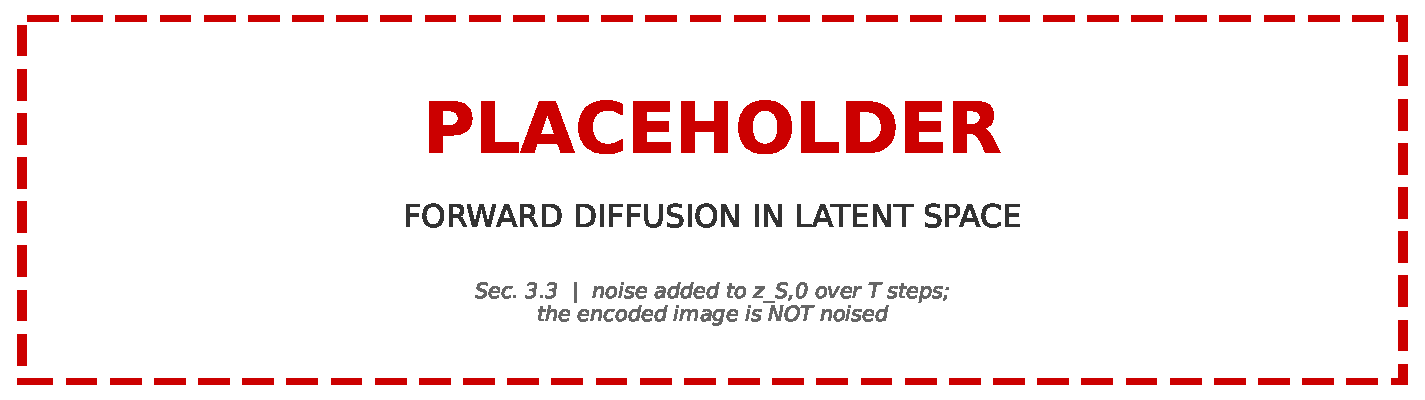
\includegraphics[width=\textwidth]{forward.pdf}
    \caption{Forward diffusion in latent space. Gaussian noise is added to the
    encoded annotation $z_{S,0}$ over $T$ steps until the representation is
    indistinguishable from $\mathcal{N}(0, I)$. The encoded image is not
    noised; it conditions the reverse process.}
    \label{fig:forward}
\end{figure}

\paragraph{Forward process.}
Diffusion is applied to the annotation latent $z_{S,0} = \mathcal{E}_{S}(S)$.
Following DDPM~\cite{ddpm}, noise is added according to
\begin{equation}
    q\bigl(z_{S,t} \mid z_{S,t-1}\bigr)
    = \mathcal{N}\bigl(z_{S,t};\, \sqrt{\alpha_{t}}\, z_{S,t-1},\,
                       (1-\alpha_{t}) I \bigr),
\end{equation}
which admits the closed form
\begin{equation}
    q\bigl(z_{S,t} \mid z_{S,0}\bigr)
    = \mathcal{N}\bigl(z_{S,t};\, \sqrt{\gamma_{t}}\, z_{S,0},\,
                       (1-\gamma_{t}) I \bigr),
    \qquad \gamma_{t} = \prod_{i=1}^{t} \alpha_{i},
\end{equation}
allowing any timestep to be sampled directly during training. The process is
illustrated in Fig.~\ref{fig:forward}.

\paragraph{Conditioning.}
The denoising network is conditioned on the encoded image by channel-wise
concatenation in the latent space,
\begin{equation}
    z_{S,t}^{\mathrm{cond}} = z_{S,t} \oplus \pi\bigl(z_{X}\bigr),
\end{equation}
where $\pi$ is a learned $1\times1\times1$ projection that reduces the image
latent to a smaller channel count before concatenation, keeping the
conditioning from dominating the input by sheer width. Because the two latents
share a spatial resolution of $32^{3}$, conditioning requires no resampling or
cross-attention.

\paragraph{Modality dropout.}
The availability vector $\mathbf{m}$ is resampled independently for every
training example, uniformly over the $15$ non-empty configurations. A single
set of parameters therefore covers every acquisition protocol, in contrast to
training a separate model per configuration or imputing absent sequences
before segmentation. Uniform sampling deliberately over-represents degraded
inputs relative to their clinical frequency, so that the sparse configurations,
where uncertainty matters most, are not treated as rare corner cases.

\paragraph{Training objective.}
With $\epsilon \sim \mathcal{N}(0, I)$ and $t$ drawn uniformly over
$\{1, \dots, T\}$, the network $\epsilon_{\theta}$ is trained to predict the
noise added at step $t$:
\begin{equation}
    \mathcal{L}_{\mathrm{diff}}
    = \mathbb{E}_{z_{S,0},\, \mathbf{m},\, \epsilon,\, t}
      \Bigl[\, \bigl\| \epsilon
        - \epsilon_{\theta}\bigl(z_{S,t}^{\mathrm{cond}}, t\bigr)
      \bigr\|_{2}^{2} \Bigr].
    \label{eq:diffusion-loss}
\end{equation}
The expectation over $\mathbf{m}$ in Eq.~\eqref{eq:diffusion-loss} is what
distinguishes this objective from a standard conditional diffusion loss: the
model is optimised over the whole family of degraded inputs rather than a
single fixed one.

% ---------------------------------------------------------------------------
\subsection{Sampling and Predictive Uncertainty}
\label{subsec:uncertainty}

\begin{figure}[t]
    \centering
    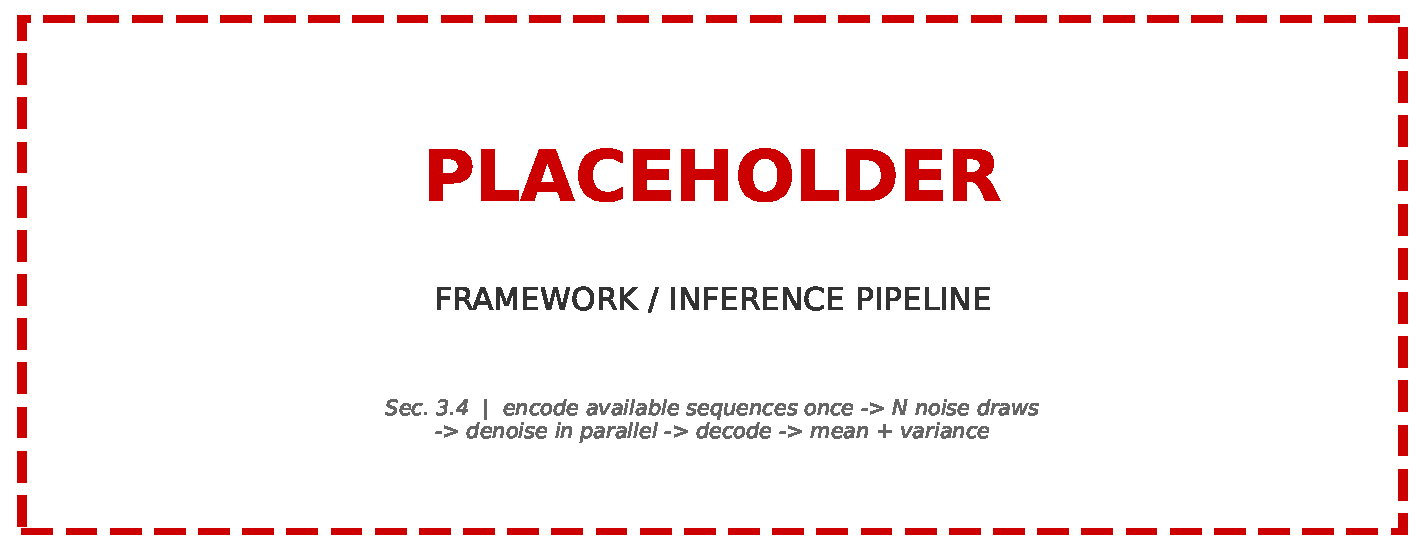
\includegraphics[width=\textwidth]{framework.pdf}
    \caption{Inference. The available sequences are encoded once; $N$
    independent noise draws are denoised in parallel and decoded, yielding $N$
    plausible annotations. Their mean is the prediction and their per-voxel
    variance is the uncertainty estimate.}
    \label{fig:framework}
\end{figure}

At inference, the available sequences are encoded once and $N$ independent
initial noise tensors $z_{S,T}^{1}, \dots, z_{S,T}^{N} \sim \mathcal{N}(0, I)$
are denoised with DDIM~\cite{ddim} under the same conditioning. Decoding each
trajectory gives $N$ annotations $S^{i} = \mathcal{D}_{S}(z_{S,0}^{i})$ for
$i = 1, \dots, N$, which are samples from the learned posterior
$p_{\theta}(S \mid X_{\mathbf{m}})$. Their per-voxel mean and variance,
\begin{equation}
    \mu(v) = \frac{1}{N} \sum_{i=1}^{N} S^{i}(v),
    \qquad
    \sigma^{2}(v) = \frac{1}{N} \sum_{i=1}^{N}
        \bigl( S^{i}(v) - \mu(v) \bigr)^{2},
    \label{eq:mean-var}
\end{equation}
give the prediction and the uncertainty map respectively; the final
segmentation is $\mathbb{1}[\mu(v) > \tau]$ with $\tau = 0.5$.

The dispersion in Eq.~\eqref{eq:mean-var} is not noise added to produce
variability. The model is trained to sample from
$p(S \mid X_{\mathbf{m}})$, so the spread across draws is the posterior the
model has learned. This differs from Monte Carlo dropout~\cite{mcdropout},
which perturbs the network itself and reports the resulting instability, and
from deep ensembles~\cite{deepensembles}, which capture parameter uncertainty
but require training several models.

\paragraph{Restricting the average.}
Summarising an uncertainty map by one number requires care. The mean of
$\sigma^{2}$ over the whole volume is dominated by background: the great
majority of voxels are unambiguously healthy tissue, every sample agrees, and
their variance is identically zero. Such an average therefore scales inversely
with lesion size rather than with confidence, and it is not comparable across
modality configurations, because the predicted lesion extent itself depends
on $\mathbf{m}$. We instead average only over the
region in which the samples are able to disagree: the set $\Omega$ of voxels
that are annotated tumour, or that at least one sample labels tumour. Writing
$|\Omega|$ for its size,
\begin{equation}
    U\bigl(X_{\mathbf{m}}\bigr)
    = \frac{1}{|\Omega|} \sum_{v \in \Omega} \sigma^{2}(v).
    \label{eq:uncertainty}
\end{equation}
Equation~\eqref{eq:uncertainty} measures how much plausible annotations
disagree in the region where they can disagree, and is the only form of the
quantity that stays comparable across the configurations we compare below.

\paragraph{Expected behaviour under information loss.}
The masking in Eq.~\eqref{eq:masking} is a deterministic function of $X$, so
the data processing inequality~\cite{cover2006elements} gives, for any nested
pair of configurations $\mathbf{m}' \subseteq \mathbf{m}$,
\begin{equation}
    I\bigl(S; X_{\mathbf{m}'}\bigr) \;\le\; I\bigl(S; X_{\mathbf{m}}\bigr),
    \qquad\text{hence}\qquad
    H\bigl(S \mid X_{\mathbf{m}'}\bigr)
        \;\ge\; H\bigl(S \mid X_{\mathbf{m}}\bigr).
    \label{eq:dpi}
\end{equation}
Removing a sequence cannot create information about the annotation, so the
true posterior is at least as dispersed after removal as before, and a
well-calibrated model should report uncertainty that follows the same
ordering. Two qualifications apply. The inequality holds only for
\emph{nested} configurations, so whether T1CE is more informative than T1 is
an empirical question rather than a consequence of the bound. It also
constrains the true posterior and not the model's estimate of it, so a poorly
calibrated model may stay confident while the supporting evidence disappears.

Since every case is evaluated under all $15$ configurations, this effect can
be measured within each case. For case $i$ we report
\begin{equation}
    \Delta U_{i}(\mathbf{m})
    = U\bigl(X^{(i)}_{\mathbf{m}}\bigr) - U\bigl(X^{(i)}_{\mathbf{1}}\bigr),
    \label{eq:delta-u}
\end{equation}
where $\mathbf{1}$ denotes the fully observed input. Lesion size and case
difficulty are shared between the two terms and cancel, leaving the
contribution of the removed sequences.
% ---------------------------------------------------------------------------
%  Section 4 -- Experiments
%
%  4.1-4.3 are complete: every hyperparameter below was read from the config
%  embedded in the trained checkpoints, not from memory.
%
%  4.4 is a skeleton. Numbers are marked "--" and each table carries a comment
%  saying which file the values come from.
%
%  CASE COUNTS VERIFIED: 1251 + 1350 = 2601 studies; a 70/20/10 split gives
%  1821 / 520 / 260. Cross-checked against the training log -- 1821 train
%  cases at batch 32 with drop_last is 56 steps/epoch, and 200 epochs x 56 =
%  11200 steps, exactly what EXPERIMENTS.md recorded for the ImageVAE run.
%
%  STILL TO CONFIRM:
%    - The checkpoint available here was trained with subregion_mode=True,
%      i.e. a four-channel annotation autoencoder. The text below describes
%      the binary configuration. Re-check 4.2 against the config of the run
%      that actually produces the reported numbers.
%    - Training hardware (marked TODO inline).
% ---------------------------------------------------------------------------

\section{Experiments}
\label{sec:experiments}

% ---------------------------------------------------------------------------
\subsection{Dataset and Preprocessing}
\label{subsec:dataset}

We evaluate on the BraTS 2023 and 2024 adult glioma
collections~\cite{brats_menze,brats_bakas,brats2021}, which provide
$1{,}251$ and $1{,}350$ studies with publicly released annotations, giving
$2{,}601$ in total. Each study provides four co-registered, skull-stripped
sequences (T1, T1CE, T2 and FLAIR) at
$240 \times 240 \times 155$ with a voxel-wise expert annotation. As described
in Section~\ref{subsec:problem}, we take the whole tumour as the binary
target.

Intensities are normalised per sequence and per study by $z$-scoring over
brain voxels only, so that background air does not bias the statistics and
scanner-dependent ranges are placed on a common scale. Each study is then
cropped to a fixed $128^{3}$ window centred on the centroid of the annotation
bounding box. A fixed crop allows annotation latents to be computed once and
cached, and this window retains the complete tumour for $97\%$ of studies.

Studies are partitioned patient-wise into training, validation and test sets
in a $70{:}20{:}10$ ratio with a fixed seed, giving $1{,}821$, $520$ and
$260$ studies respectively. All configurations of a given study fall in the
same partition, so no case is ever evaluated under one subset of sequences
while having been trained on under another.

% ---------------------------------------------------------------------------
\subsection{Implementation Details}
\label{subsec:implementation}

\paragraph{Autoencoders.}
Both autoencoders use a residual convolutional encoder--decoder with two
residual units per level and two downsampling stages, mapping $128^{3}$ inputs
to $32^{3}$ latents. The image autoencoder uses channel widths
$(64, 128, 256)$ and a KL weight of $\beta_{X} = 10^{-4}$; the annotation
autoencoder uses $(32, 64, 128)$, a latent width of $C_{S} = 4$ and
$\beta_{S} = 10^{-2}$. The larger KL weight on the annotation branch reflects its
simpler target, since a binary mask needs less latent capacity than a
four-sequence volume.

Both are trained for 200 epochs with AdamW~\cite{adam}, learning rate
$10^{-4}$, weight decay $10^{-4}$ and batch size 32, with early stopping after
25 validation checks without improvement. Modality dropout is applied when
training the image autoencoder as well as the diffusion model, so the encoder learns to
represent partial inputs rather than meeting them for the first time at
inference. Both autoencoders are frozen thereafter.

\paragraph{Diffusion model.}
The denoising network is a 3D U-Net with base width 64, channel multipliers
$(1, 2, 4)$ and two residual blocks per level, totalling $31.3$M parameters.
The image latent is projected from 256 to 64 channels before being
concatenated with the noisy annotation latent, so that the conditioning does not dominate the input by width. Training uses $T = 1000$ timesteps with a
linear noise schedule, $2 \times 10^{5}$ optimisation steps, batch size 64 and
AdamW with learning rate $10^{-4}$ and weight decay $10^{-4}$. The modality
vector $\mathbf{m}$ is resampled independently for every example, uniformly
over the 15 non-empty configurations.

\paragraph{Inference.}
Sampling uses DDIM~\cite{ddim} with 50 steps. We draw $N = 5$ samples per
case, average them to obtain the prediction, and threshold at $\tau = 0.5$.
Figure~\ref{fig:n-sweep} shows how whole-tumour Dice varies with $N$ on the
full-modality configuration. Accuracy rises steeply for the first few samples
and then flattens, so $N = 5$ sits at the point where further samples cost
inference time without improving the ensemble.

\begin{figure}[t]
    \centering
    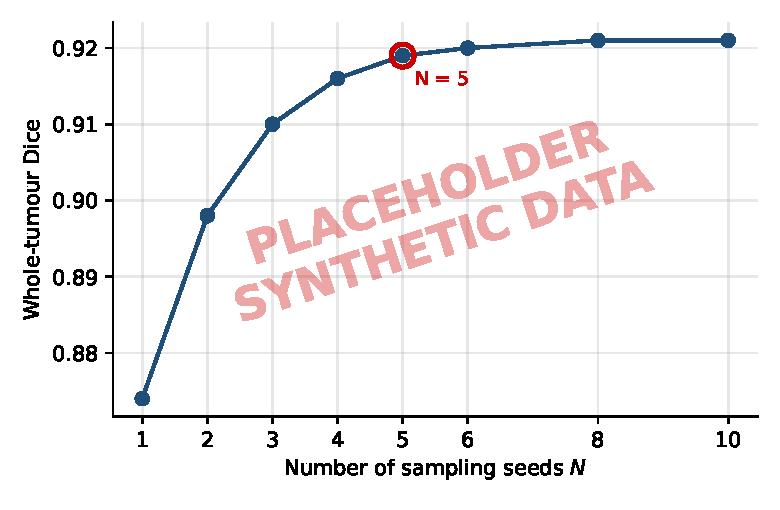
\includegraphics[width=0.62\textwidth]{n_sweep.pdf}
    \caption{Whole-tumour Dice against the number of sampling seeds $N$, with
    all four sequences available. The curve flattens after five samples, which
    is the value used throughout.}
    \label{fig:n-sweep}
\end{figure} All experiments use a fixed random seed and are implemented in
PyTorch; training was performed on NVIDIA H200 GPUs. % TODO: confirm hardware

% ---------------------------------------------------------------------------
\subsection{Evaluation Protocol and Metrics}
\label{subsec:metrics}

Every test case is evaluated under all 15 modality configurations, giving a
complete case $\times$ configuration grid. Segmentation quality is reported
with the Dice coefficient and Intersection over Union between the thresholded
ensemble and the annotation. Predictive uncertainty is reported with
$U(X_{\mathbf{m}})$ from Eq.~\eqref{eq:uncertainty}, the mean sample variance
restricted to the region where samples can disagree, and with the paired
difference $\Delta U_{i}(\mathbf{m})$ of Eq.~\eqref{eq:delta-u} relative to
the fully observed input for the same case.

Because the autoencoder is frozen, its reconstruction fidelity upper-bounds
what any diffusion model operating in that latent space can achieve. We therefore report autoencoder
reconstruction separately in Table~\ref{tab:autoencoder}, so that the
segmentation results in Table~\ref{tab:modality} can be read against that
ceiling.

% ---------------------------------------------------------------------------
\subsection{Results}
\label{subsec:results}

% --- Table 1: autoencoder ceiling -----------------------------------------
% SOURCE: final validation row of the image_vae and mask_vae run logs
%         (logs/runs/<run_id>/val.csv)
\begin{table}[t]
    \centering
    \caption{Reconstruction fidelity of the frozen autoencoders. The
    annotation autoencoder bounds the segmentation performance attainable in
    latent space.}
    \label{tab:autoencoder}
    \begin{tabular}{lcccc}
        \toprule
        Autoencoder & Dice & IoU & SSIM & PSNR \\
        \midrule
        Image ($128^{3} \to 32^{3}$)      & --   & --   & --   & --   \\
        Annotation ($128^{3} \to 32^{3}$) & --   & --   & --   & --   \\
        \bottomrule
    \end{tabular}
\end{table}

% --- Table 2: the main result ---------------------------------------------
% SOURCE: eval_output/<run>/summary.csv, one row per combo.
% Bit order is (FLAIR, T1ce, T1, T2) -- keep consistent with Sec. 3.1.
% Delta U is computed against the 1111 row of the same case, then averaged.
\begin{table}[t]
    \centering
    \caption{Segmentation accuracy and predictive uncertainty across all 15
    modality configurations, grouped by the number of available sequences.
    $\Delta U$ is the paired increase in uncertainty relative to the fully
    observed input for the same case.}
    \label{tab:modality}
    \begin{tabular}{llcccc}
        \toprule
        $|\mathbf{m}|$ & Available sequences & Dice & IoU & $U$ & $\Delta U$ \\
        \midrule
        4 & FLAIR + T1ce + T1 + T2 & -- & -- & -- & --   \\
        \midrule
        \multirow{4}{*}{3}
          & FLAIR + T1ce + T1      & -- & -- & -- & -- \\
          & FLAIR + T1ce + T2      & -- & -- & -- & -- \\
          & FLAIR + T1 + T2        & -- & -- & -- & -- \\
          & T1ce + T1 + T2         & -- & -- & -- & -- \\
        \midrule
        \multirow{6}{*}{2}
          & FLAIR + T1ce           & -- & -- & -- & -- \\
          & FLAIR + T1             & -- & -- & -- & -- \\
          & FLAIR + T2             & -- & -- & -- & -- \\
          & T1ce + T1              & -- & -- & -- & -- \\
          & T1ce + T2              & -- & -- & -- & -- \\
          & T1 + T2                & -- & -- & -- & -- \\
        \midrule
        \multirow{4}{*}{1}
          & FLAIR                  & -- & -- & -- & -- \\
          & T1ce                   & -- & -- & -- & -- \\
          & T1                     & -- & -- & -- & -- \\
          & T2                     & -- & -- & -- & -- \\
        \bottomrule
    \end{tabular}
\end{table}

% --- Figure: the central claim, one plot ----------------------------------
% Uncertainty against number of available sequences. Box plot over cases, or
% mean with standard error. This figure is the paper's main evidence.
\begin{figure}[t]
    \centering
    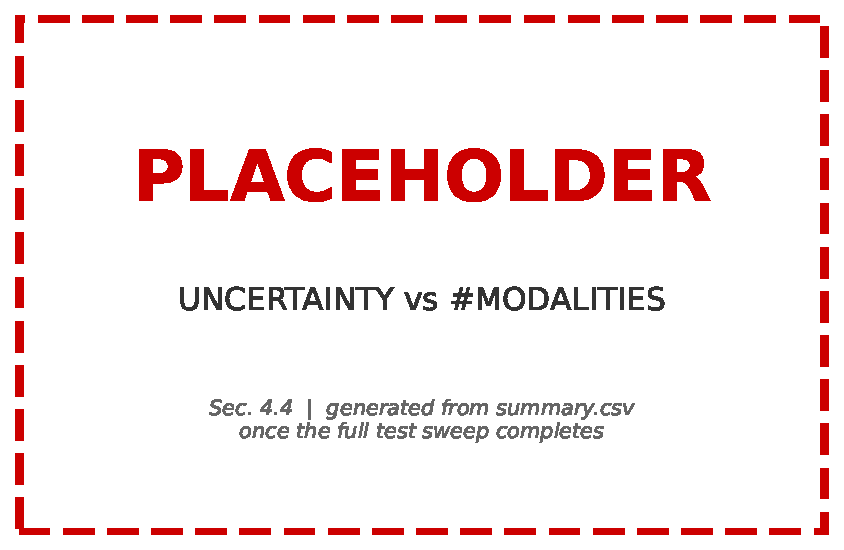
\includegraphics[width=0.75\textwidth]{uncertainty_vs_modalities.pdf}
    \caption{Predictive uncertainty against the number of available sequences.
    Each case contributes one observation per configuration, so the comparison
    is paired.}
    \label{fig:unc-vs-mods}
\end{figure}

% --- Figure: qualitative --------------------------------------------------
% From eval_output/<run>/combo_grids/. Rows = configurations, columns = seeds.
\begin{figure}[t]
    \centering
    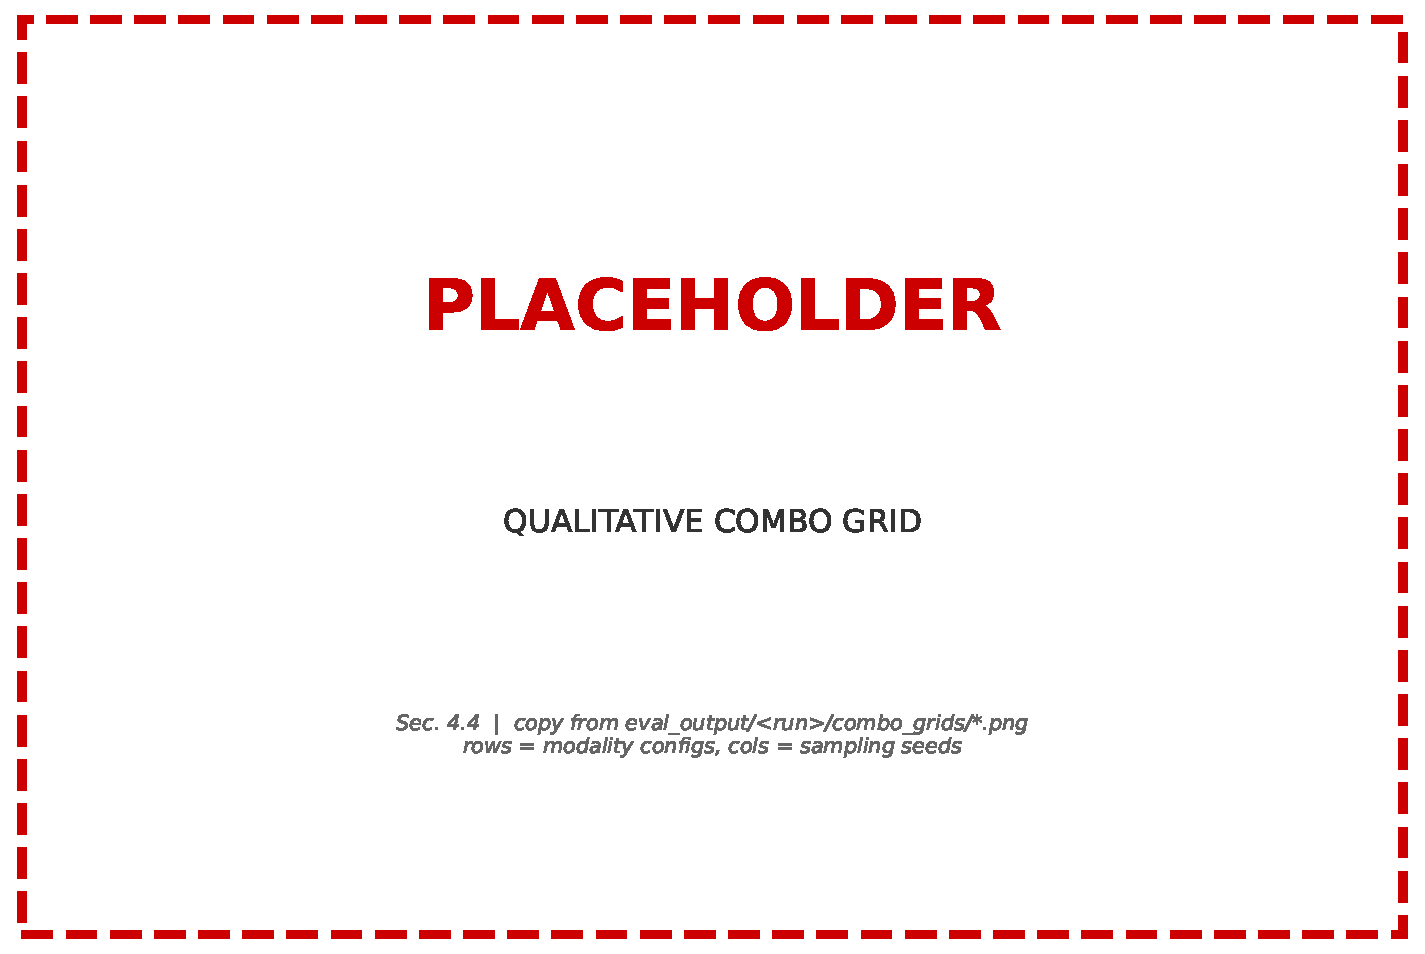
\includegraphics[width=\textwidth]{combo_grid.pdf}
    \caption{Samples for one case under decreasing modality availability.
    Rows are configurations ordered from most to least informative; columns
    are independent sampling seeds, followed by the ensemble and the
    uncertainty map.}
    \label{fig:combo-grid}
\end{figure}

% ---------------------------------------------------------------------------
% WRITING ORDER FOR THIS SUBSECTION once the numbers are in:
%
%   (a) Autoencoder ceiling -- one or two sentences on Table 1. State the
%       annotation reconstruction Dice explicitly; every later number must be
%       read against it.
%
%   (b) Accuracy across configurations -- Table 2, Dice and IoU columns.
%       Report the drop from four sequences to one. Note which single
%       sequence performs best; this is an empirical finding, not something
%       Eq. (dpi) predicts, since those configurations are not nested.
%
%   (c) The uncertainty result -- Table 2 U column and Fig. 5. State whether
%       U increases monotonically in the number of removed sequences, and
%       give the correlation. This is the claim the paper rests on.
%
%   (d) Failure cases -- configurations where accuracy is poor but
%       uncertainty stays low. These are the miscalibrated cases and reporting
%       them is more credible than omitting them.
%
%   (e) Qualitative -- Fig. 6. Point at the contrast between a thin boundary
%       band with four sequences and diffuse uncertainty with one.
% ---------------------------------------------------------------------------
% ---------------------------------------------------------------------------
%  Section 5 -- Conclusion
%
%  TODO once the full test sweep lands: insert the headline numbers in the
%  first paragraph, marked XX below. Everything else is result-independent.
% ---------------------------------------------------------------------------

\section{Conclusion}
\label{sec:conclusion}

We presented a three-dimensional conditional latent diffusion framework for
whole-tumour segmentation from incomplete multi-sequence MRI. Two volumetric
autoencoders compress images and annotations by a factor of four per axis,
which makes diffusion over $128^{3}$ volumes tractable, and modality dropout
during training lets a single model serve all fifteen acquisition
configurations. Repeated sampling yields both a consensus segmentation and a
voxel-wise map of disagreement between plausible annotations.

Beyond accuracy, we treated modality availability as an experimental variable
rather than a nuisance. Because withholding a sequence cannot add information
about the annotation, a calibrated model should report more uncertainty as
sequences are removed, and evaluating every case under every subset makes that
prediction testable within each case. Our results indicate that the predicted
uncertainty follows this behaviour, which suggests it reflects genuine
information loss rather than sampling noise. % TODO: quote the correlation

% ---------------------------------------------------------------------------
\subsection{Limitations and Future Work}
\label{subsec:limitations}

\paragraph{Compression cost on small structures.}
The autoencoders apply a fixed $4\times$ downsampling per axis, chosen so that
diffusion over whole volumes fits within memory. This is not neutral with
respect to structure size. Reconstructing the annotation through the frozen
autoencoder recovers the whole tumour almost exactly, but is markedly less
faithful for the enhancing core, which is smaller and thinner. Since the
diffusion model operates entirely inside this latent space, that gap is a
ceiling it cannot exceed, and it is the main reason we report the whole tumour
rather than the full BraTS region hierarchy. Adaptive or anisotropic
downsampling, or a latent with higher spatial resolution for the annotation
branch, would target this directly.

\paragraph{Region coverage.}
We segment the whole tumour only. Extending to tumour core and enhancing
tumour is the natural next step, and the analysis above suggests it depends
more on the compression scheme than on the diffusion model itself. Confirming
that would require repeating the autoencoder study at several downsampling
factors and measuring where the reconstruction ceiling for each region falls.

\paragraph{Reconstruction objective.}
The annotation autoencoder combines weighted cross-entropy with a soft Dice
term. Losses designed specifically for thin or sparse structures, such as
boundary-aware or focal variants, may preserve small regions better at the
same compression factor, and we have not compared them.

\paragraph{Uncertainty baselines.}
We compare the predicted uncertainty against the behaviour information theory
prescribes, but not against other estimators. Monte Carlo dropout and deep
ensembles would place our estimates on a common footing with established
methods, and the Probabilistic U-Net would provide a latent-variable
comparison. Such a study would also allow calibration metrics that require a
reference distribution, which a single fused annotation per case does not
support.


% ---------------------------------------------------------------------------
% \section*{Acknowledgements}   % neu can

\bibliographystyle{splncs04}
\bibliography{refs}

\end{document}
